\documentclass{article}


\usepackage[english]{babel}
\usepackage{graphicx}
\usepackage{hyperref}    % for clickable links
\usepackage{subcaption}  % for subfigures

% Set page size and margins
% Replace `letterpaper' with `a4paper' for UK/EU standard size
\usepackage[letterpaper,top=2cm,bottom=2cm,left=3cm,right=3cm,marginparwidth=1.75cm]{geometry}

% Useful packages
\usepackage{amsmath}
\usepackage{graphicx}
\usepackage[colorlinks=true, allcolors=blue]{hyperref}





\title{Problem Set 6}
\author{Caleb Reid}


\begin{document}

\maketitle

I grabbed Rainbow Six Siege data from  
\href{https://www.kaggle.com/code/cmsrinivas0/rainbow-six-seige-data-analysis}{Kaggle}. 
I am interested in the data because I like playing and watching R6 Siege, and I enjoy looking at stats. 
The data was supplied by Ubisoft and therefore was pre-cleaned. I examined the data using ggplot2 and gt packages in RStudio.


% --- First Image ---
\begin{figure}[h!]
    \centering
    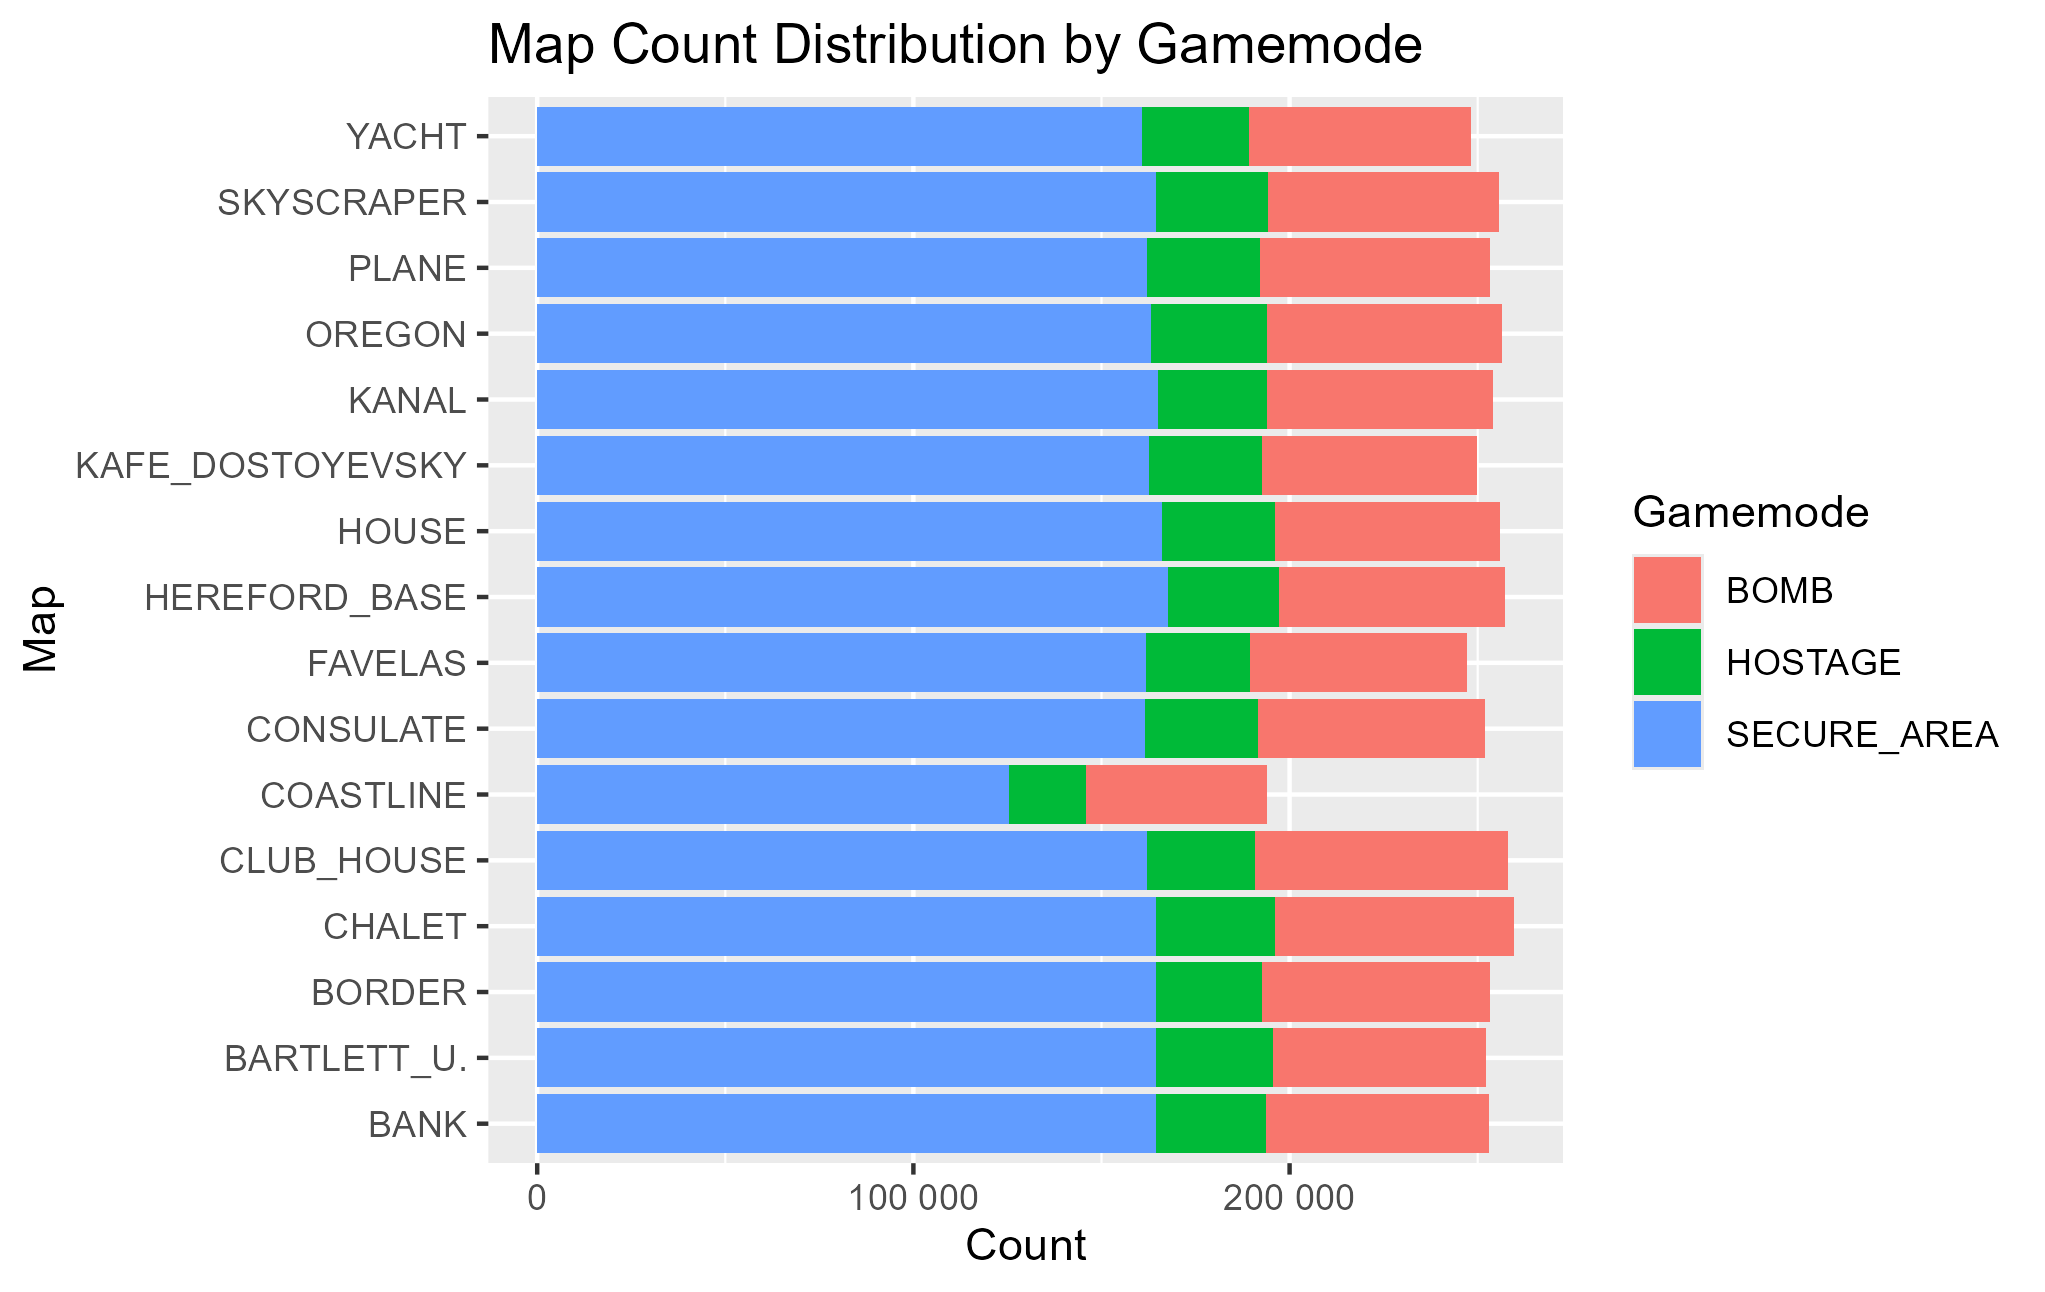
\includegraphics[width=0.9\textwidth]{PS6a_Reid.png}
    \caption{PS6a Figure}
    \label{fig:PS6a}
\end{figure}

% --- Second Image ---
\begin{figure}[h!]
    \centering
    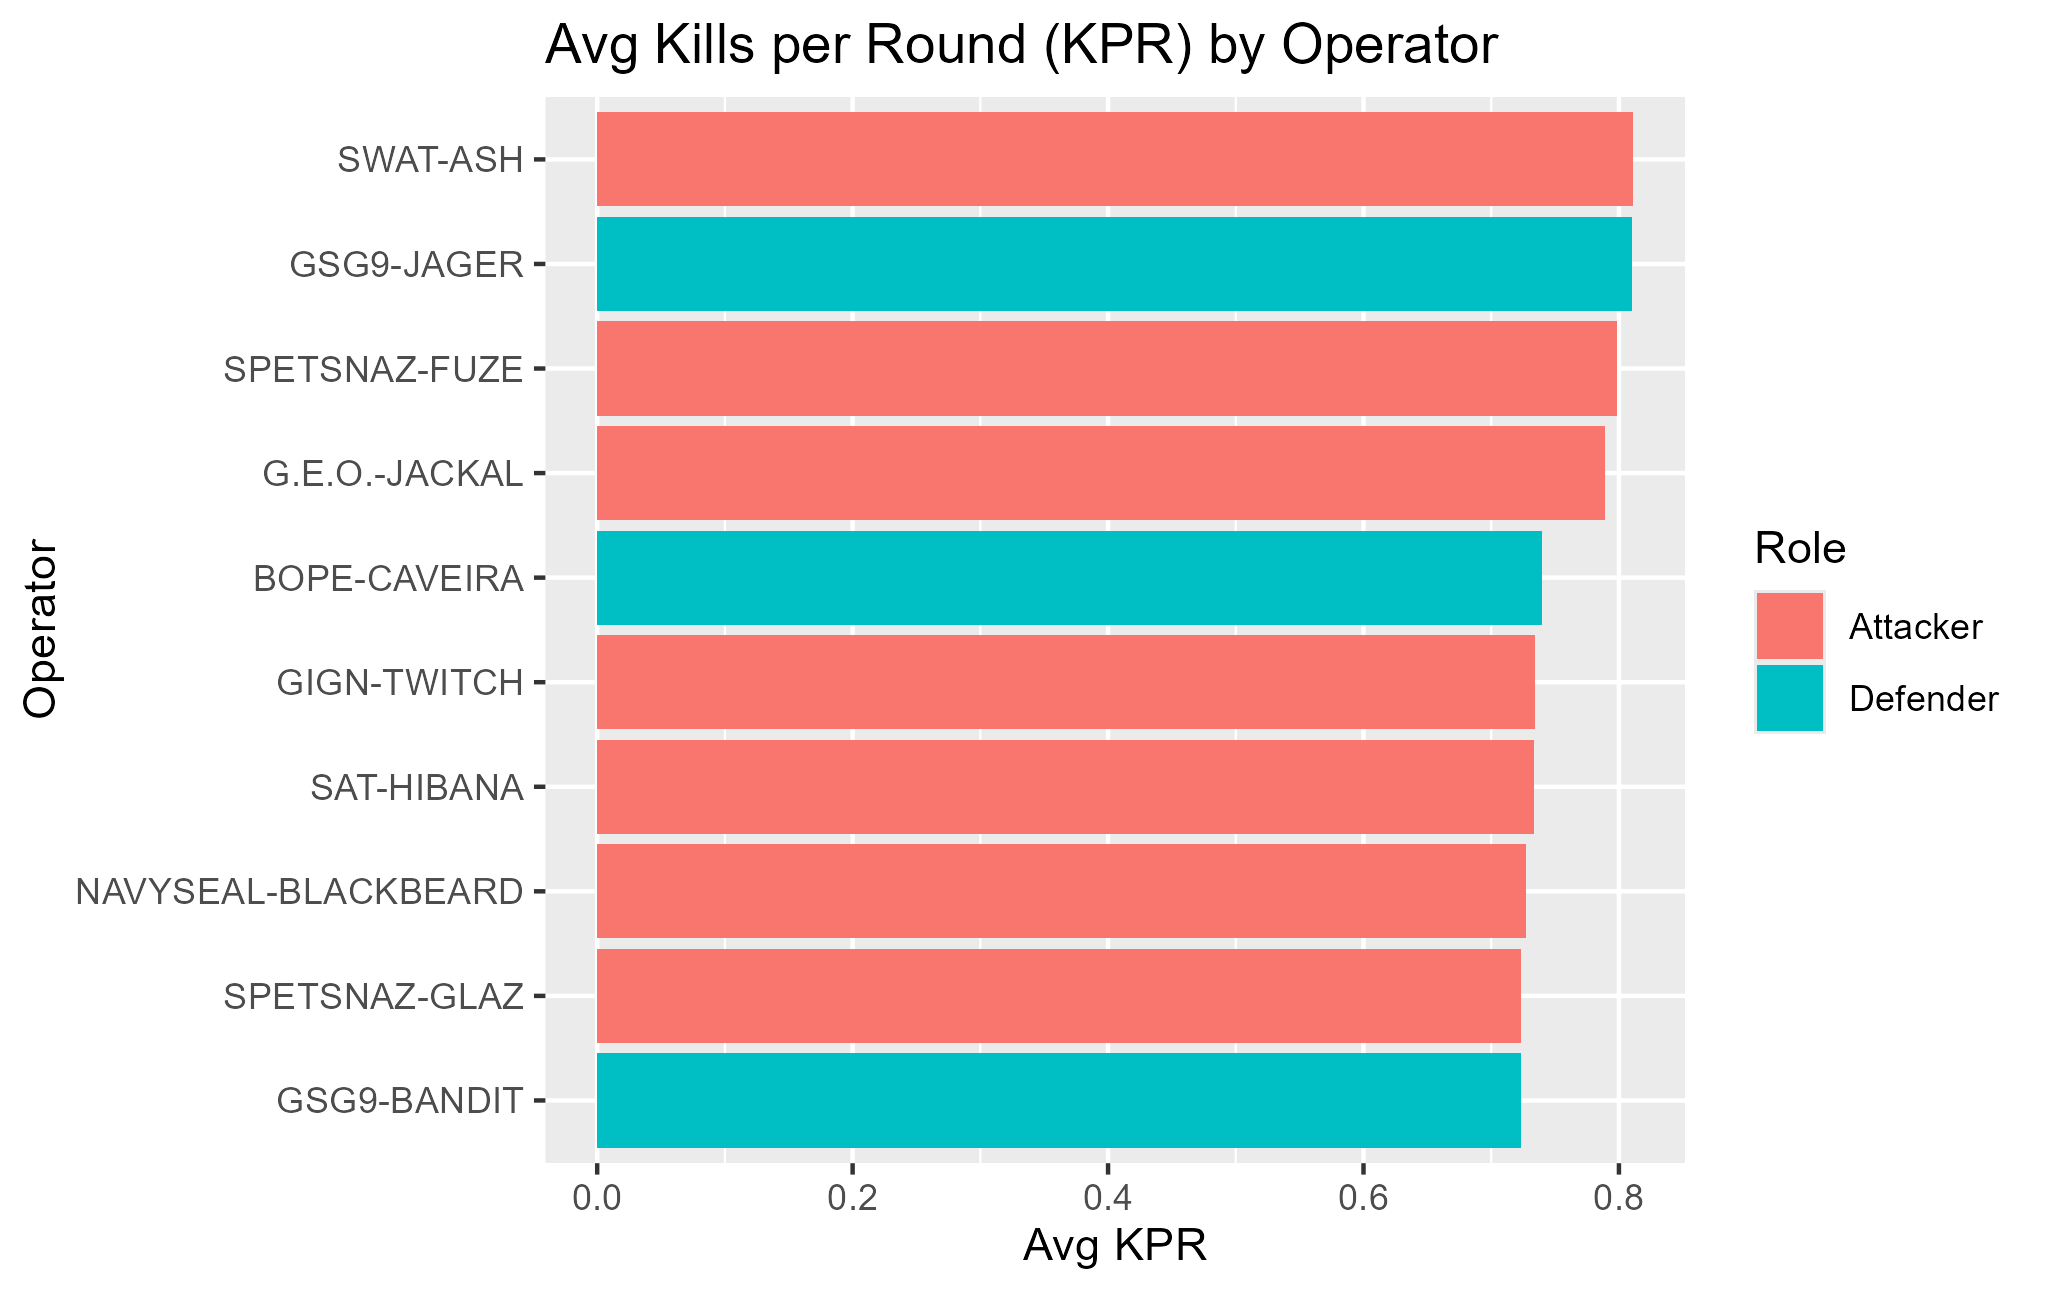
\includegraphics[width=0.9\textwidth]{PS6b_Reid.png}
    \caption{PS6b Figure}
    \label{fig:PS6b}
\end{figure}

% --- Third Image ---
\begin{figure}[h!]
    \centering
    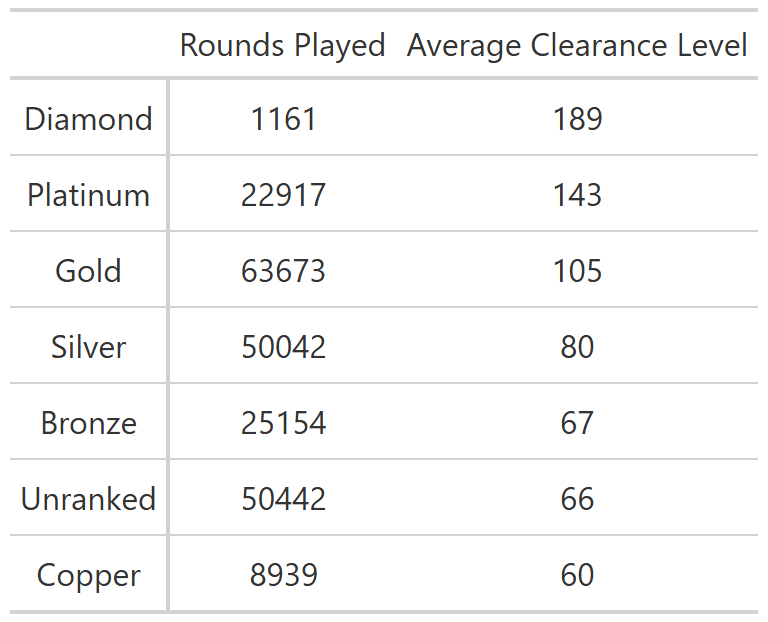
\includegraphics[width=0.9\textwidth]{PS6c_Reid.png}
    \caption{PS6c Figure}
    \label{fig:PS6c}
\end{figure}

\end{document}

\end{document}
